
% \paragraph{ \( \Phi \) }
%
% \begin{equation}
%   \Phi(r) = - \frac{4\pi G \rho_0 R_s^3}{r} \ln ( 1+ \frac{r}{R_s} )
% \end{equation}
%
% with the limits
%
% \begin{equation}
%   \lim_{r\to \infty} \Phi=0
% \end{equation}
%
% and
%


\subsection{Generierung der Elliptischen Galaxien}
\subsubsection{Das Navarro-Frenk-White Profil}

Das Navarro-Frenk-White profil (NFW-profil) ist im grunde genommen eine Funktion
die einem die Warscheinlichkeit das ein Stern an einer bestimmten position ist
liefert.
Die Funktion ist im allgemeinen wie folgt aufgebaut:

\begin{equation} \label{eq:NFW_profile}
  \rho_{NFW}(r) = \frac{ 1 }{ \sqrt{ 2 \pi } \cdot \sigma } \cdot
  \exp \left( \frac{ -\phi(r) }{ \sigma^{ 2 } } \right)
\end{equation}

\begin{equation*}
  \phi(r) = \frac{ 4\pi \cdot G \cdot f_{0} \cdot R_{s}^3 }{ r } \cdot
  ln{ \left( 1 + \frac{ r }{ R_{s} } \right) }
\end{equation*}

Um die Formel (\ref{eq:NFW_profile}) einfach zu beschreiben kann man sie sich
wie folgt vorstellen:
Um zu gucken ob ein zufälliger Stern
bei \( x_1 \), \( y_1 \) und \( z_1 \) generiert werden kann wird wie folgt
vorgegangen: Aus den Koordinaten wird der Wert \( r \) mithilfe des Satz des
Pytargoras berechnet ( \( r = \sqrt{{x_1}^2 + {x_2}^2 + {x_3}^2} \) ) , dieser gibt
an wie weit der jeweilige Stern vom Zentrum der Galaxie entfernt ist. Um zu
prüfen ob der Stern generiert wird, wird dieser \( r \)-wert in die Funktion
\( \rho_{NFW} \) eingesetzt. Der entstehende Wert gibt an wie warscheinlich es ist,
das ein Stern in der Entfernung zum Ursprung generiert wird.

\subsubsection{Random Sampling}

Die sogennante ''Random Sampling`` Methode wird genutzt um herrauszufinden ob
ein Stern generiert wird oder nicht.Es wird dazu ein zufälliger
Wert \( x \) im bereich \( [~\rho_{max}~;~\rho_{min}~] \) generiert. Liegt dieser
Wert über dem Wert aus der Funktion \( \rho \) wird kein Stern generiert.
Liegt dieser Stern jedoch unter dem wert aus der \( \rho \) Funktion wird
ein Stern an den Koordinaten \( x_1 \), \( y_1 \) und \( z_1 \) generiert.

Um das generieren zu Beschleunigen wird eine sogenneante ''lookuptable``
verwendet. (\( \rightarrow \) \ref{subsec:lookuptable})

Generiert man ein paar Sterne mithilfe des NFW-Profils hat man theoretisch
schon eine Galaxie, jedoch ist diese nicht klar definiert. Um eine klare
definition zu erreichen müssen mehrere hundert Sterne generiert werden.

% \subsubsection{Das Einasto Profil}
%
% \begin{equation}
%   \gamma(r) = \frac{ d \ln(\rho(r)) }{ d \ln(\rho) } \propto r^{\alpha}
% \end{equation}

% \subsubsection{Blender + Python}
%
% Blender is Awesome, Python is Awesome and together they are
% \bold{SUPER AWESOME!!!}
%
% \begin{enumerate}
%   \item Generate the galaxy-data using the NFW-Profile or the Einasto-profile
%   \item Display the data in Blender and create an image using the OpenGL-renderer
%   \item Train a Neural Network (NN) to classify galaxies
%   \item Let the NN modify the galaxy to generate a perfect galaxy
% \end{enumerate}


\subsection{Generierung eines Dunkle-Materie Halos}

Das sogennannte ''Dunkle-Materie Halo`` ist eine art Kugel die eine Galaxie
umspannt: Duch dieses Halo ist die Dichte der Dunklen Materie welches sich um die
Galaxie herum befindet definiert. Problematisch ist jedoch, dass wir dieses
Halo nicht sehen können weshalb wir nur aufgrund anderer phänomäne welche durch
die Halos verursacht werden auf die Eigenschaften des Halos schließen können.
\par
Um diese Halos darzustellen wird das NFW-Profil~(\ref{eq:NFW_profile})
abgewandelt und quasi mit dem Profil für Elliptische Galaxien verbunden.

...

\subsubsection{Anpassung des NFW-Profils}

\begin{equation}
  \rho(r) = \frac{1}{\sqrt{2 \cdot \pi} \cdot \sigma} \cdot
  e^{\left( - \frac{(\Phi(r)}{\sigma^{2}} \right)}
\end{equation}

\begin{equation}
  \rho(r) \cdot 1-\frac{1}{(2 \cdot sigma^{2} )} \cdot
  ( Mxx \cdot x^{2} + 2 \cdot Mxy \cdot xy + Myy \cdot y^{2} ))
\end{equation}

\begin{lstlisting}

# new rho function
def rho_new(x, y, z):
  a = (1 - ((1) / (2 * (sigma ** 2)))
  b = ( Mxx * x**2 + 2 * Mxy * x * y + Myy * y**2 ) )
  c = a * b
return rho(x, y, z) * c

# phi function
def phi(x):
  if x == 0:
    return -4 * pi * f_0 * G * R_s**2

  a = - ( 4 * pi * G * f_0 * R_s ** 3 ) / x
  b = np.log(1. + (x / R_s) )
  c = a * b
  return c

\end{lstlisting}


\subsection{Stauchung und Streckung der Galaxie}

Wird eine Galaxie gestreckt oder gestaucht kann das an der umliegenden Dunklen
Materie liegen. Um solch eine Streckung darzustellen wird wie folgt vorgegangen:
Die Position eines Sternes an einer Achse muss mit einem Skalar multipliziert
bzw. dividiert werden.
Dies ist relativ einfach machbar da die Koordinaten der jeweiligen Sterne
in einer Datei nach dem Format \( [x, y, z] \) gespeichert sind.
Um die Galaxie vertikal zu strecken wird z.B. für jeden Stern die z-Koordinate
mit dem skalar \( s \) multipliziert. Da gestaucht werden soll liegt dieser
Wert im Intervall \( 0 < s < 1 \). Die neue Koordinate für einen Stern ist also
\( [x, y, z \cdot s] \). Möchte man die Galaxie strecken muss das Skalar \( s \)
im Intervall \( 1 < s < \infty \) liegen.

\subsection{Beschleunigung der Generierung}

Die Sterne schnell zu generieren ist natürlich energieeffizienter aber auch
wichtig damit das neuronale netzt in unserer lebzeit fertig wird.

Es gibt ein paar Aktionen die umgebaut werden können um das generieren zu
beschleunigen:

\subsubsection{n-Sterne}

Statt am Anfang mehrere Millionen Sterne zu generieren wird wenn eine
neue Koordinate benötigt wird eine neue erstellt. So erstellt man auf keinen
Fall zu viele Koordinaten was Zeit spaart.
Dem programm kann also gesagt werden, dass es genau \( n_1 \) Sterne aus
\( m_1 \) potentiellen Sternen generieren soll, andernfalls werden \( n_2 \)
Sterne aus \( m_2 > m_1 \) potentiellen Sternen generiert.

\subsubsection{Lookuptable} \label{subsec:lookuptable}

Eine Weitere Möglichkeit für meherere Berechnungen Zeit zu Spaaren ist, den
Entsprechenden Wert aus dem NFW-Profil (Formel \ref{eq:NFW_profile}) vorher zu
berechnen und in eine Tabelle zu schreiben.
Dies kann für z.B. \( 2e8 \) Werte getan werden was zwar eine 6 GB große Datei
erzeugt, diese kann jedoch innerhalb weniger Sekunden eingelesen werden.

\subsubsection{Weitere Optimierungen}

\paragraph{Nichts in der Konsole ausgeben:}

Eine Vorgang der erstaunlicherweise sehr viel Rechenleistung erfordert, ist
der Vorgang beim ausgeben von Text in die Konsole. Gibt man jede potentielle
Koordinate in die Konsole aus, stürtzt das Programm aufgund von Überlast ab.
Um dies zu umgehen kann z.B. nur jeder 100.000 Wert in die Konsole ausgegeben
werden.

\paragraph{...}

\newpage
\subsection{Nutzung eines Neuronalen Netzes zum unbeaufsichtigeten generieren}
\subsubsection{Aufbau des Neuronalen Netzes}

Ein Neuronales Netz ist wie folgt aufgebaut:

\bigskip

\hrule

\bigskip

\tikzset{%
  every neuron/.style={
    circle,
    draw,
    minimum size=1cm
  },
  neuron missing/.style={
    draw=none,
    scale=2,
    text height=0.333cm,
    execute at begin node=\color{black}$\vdots$
  },
}

\begin{center}
  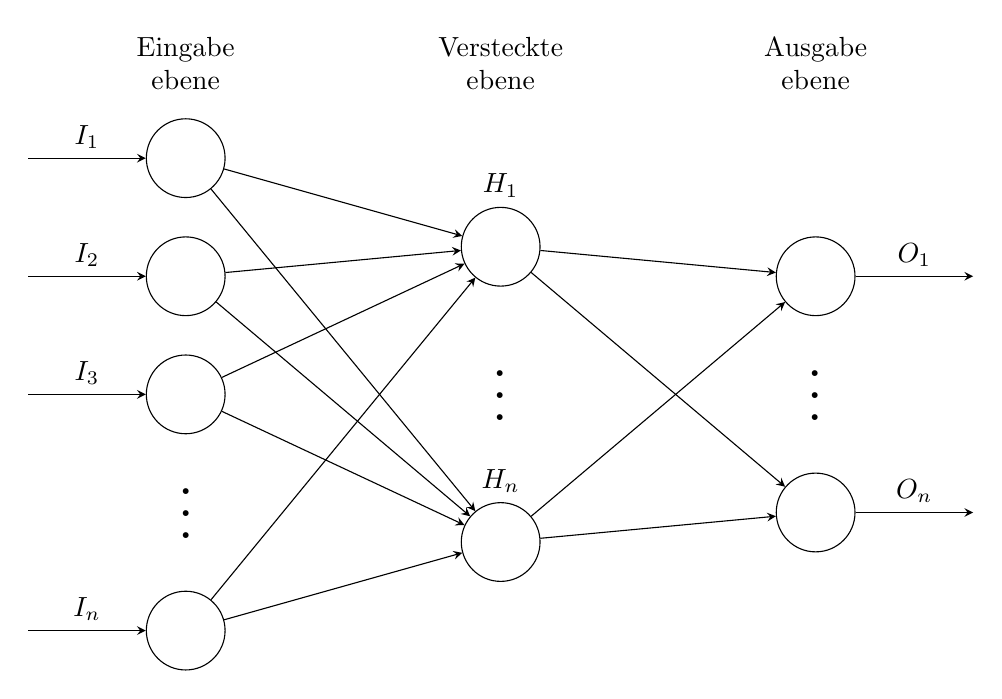
\begin{tikzpicture}[x=2cm, y=1.5cm, >=stealth]

  \foreach \m/\l [count=\y] in {1,2,3,missing,4}
    \node [every neuron/.try, neuron \m/.try] (input-\m) at (0,2.5-\y) {};

  \foreach \m [count=\y] in {1,missing,2}
    \node [every neuron/.try, neuron \m/.try ] (hidden-\m) at (2,2-\y*1.25) {};

  \foreach \m [count=\y] in {1,missing,2}
    \node [every neuron/.try, neuron \m/.try ] (output-\m) at (4,1.5-\y) {};

  \foreach \l [count=\i] in {1,2,3,n}
    \draw [<-] (input-\i) -- ++(-1,0)
      node [above, midway] {$I_\l$};

  \foreach \l [count=\i] in {1,n}
    \node [above] at (hidden-\i.north) {$H_\l$};

  \foreach \l [count=\i] in {1,n}
    \draw [->] (output-\i) -- ++(1,0)
      node [above, midway] {$O_\l$};

  \foreach \i in {1,...,4}
    \foreach \j in {1,...,2}
      \draw [->] (input-\i) -- (hidden-\j);

  \foreach \i in {1,...,2}
    \foreach \j in {1,...,2}
      \draw [->] (hidden-\i) -- (output-\j);

  \foreach \l [count=\x from 0] in {Eingabe, Versteckte, Ausgabe}
    \node [align=center, above] at (\x*2,2) {\l \\ ebene};

  \end{tikzpicture}
\end{center}
\bigskip

\hrule

\bigskip

Das \textbf{Neuronale Netz} besitze mehrere Ebenen: die \textbf{Eingabe ebene},
die \textbf{Versteckte Ebene(n)} und die \textbf{Ausgabe Ebene}.
Diese Ebenen bestehen aus sogennanten \textbf{Neuronen} die wie im Menschlichen
Gehirn Informationen aufnehmen und weitergeben. Die Eingabe kann verschieden
gewichtet sein, es kann also sein das eine Eingabe eine Gewichtung von
\( 10\% \) hat und eine andere eine Gewichtung von \( 90\% \).
Die Eingabe Ebene ist dazu da eine Eingabe inform einer Matrix an die
verschiedenen Neuronen in der Versteckten Ebene weiterzuleiten.
Die Versteckte Ebene verarbeitet die Information aus der Matrix und leitet
diese an die Ausgabe Ebene weiter die die Information ausgibt.
\par
Das sogennante ''Trainieren`` ist der Prozess, bei dem die Gewichtung der
Neuronen so Verändert wird, damit ein gewünschtes Ergebnis herrauskommt.
Beispiel: man möchte ein Neuronales Netz darauf Trainieren eine Galaxie zu
Identifizieren, dann werden ganz viele positiv Beispiele durch das Netz gejagt
welche die Gewichtung immer weiter anpassen. In der Ausgangs Ebene wird dann
mithilfe zweier Neuronen entweder dargestellt das das eingegebene Bild eine
Galaxie ist oder das das eingegebene Bild eben keine Galaxie ist.

\subsubsection{Nutzung eines Neuronalen Netztes zur verbesserung von Galaxien Simulationen}

Möchte man mithilfe eines Neuronalen Netztes vorhandene Galaxiensimulationen
verbessern, wird wie im folgenden Diagramm zusehen vorgegangen:

\begin{tikzpicture}
[node distance = 4cm, auto, ->, on grid]

\node [draw, minimum width=3cm, text depth = 1cm] (galaxy) {Galaxie};
\node [draw, right of=galaxy] (neural_net) {Neuralonales Netz};

\node [draw] (yes) [right of=neural_net] {Ja}
node [right=3cm of yes, align=center] {Galaxie ist eine Galaxie};

\node [draw] (no) [below=2cm of neural_net] {Nein}
node [right=3.5cm of no, align=center] {Galaxie ist keine Galaxie \\
\( \rightarrow \) ändere parameter und \\generiere eine neue Galaxie};


\draw[->, line width=0.25mm] (galaxy) -- (neural_net)
node [above=1cm of neural_net, align=center] {Testet ob die Eingabe \\eine
Galaxie ist oder nicht};

\node[draw, yshift=5mm] (paramter) at (galaxy.south) {paramter};

\draw[->, line width=0.25mm] (neural_net) -- (yes);
\draw[->, line width=0.25mm] (neural_net) -- (no);

\path[line width=0.25mm] (no) edge [bend left] node {} (paramter);

\end{tikzpicture}

\subsection{Spiralgalaxien}
\subsubsection{Das n-Körper Problem}

\subsection{Größeneinheiten}

\begin{equation}
  3.086 \cdot 10^{36} m
\end{equation}
